\documentclass[conference]{IEEEtran}

% ---- Packages ----
\usepackage{amsmath,amssymb,amsfonts}
\usepackage{algorithmic}
\usepackage{graphicx}
\usepackage{textcomp}
\usepackage{booktabs}
\usepackage{multirow}
\usepackage{cite}
\usepackage{xcolor}
\usepackage{url}
\usepackage{balance}
\usepackage{array}
\usepackage{makecell}
\usepackage[ruled,vlined,linesnumbered]{algorithm2e}
\usepackage{subcaption}
\usepackage{tikz}
\usetikzlibrary{arrows.meta,positioning,shapes.geometric,fit,calc}

% compact lists
\usepackage{enumitem}
\setlist{nosep,leftmargin=*}

% ---- Custom commands ----
\newcommand{\ie}{\textit{i.e.}}
\newcommand{\eg}{\textit{e.g.}}
\newcommand{\etal}{\textit{et al.}}
\newcommand{\vomega}{\boldsymbol{\omega}}
\newcommand{\vpsi}{\boldsymbol{\psi}}
\newcommand{\vr}{\mathbf{r}}
\newcommand{\vs}{\mathbf{s}}
\newcommand{\Real}{\mathbb{R}}

\newtheorem{definition}{Definition}
\newtheorem{proposition}{Proposition}

% ---- Placeholder for expected results ----
\newcommand{\TBD}[1]{{\color{blue!70!black}\textbf{[#1]}}}

\begin{document}

\title{PCF-MORL: Multi-Objective QoS Optimization for\\5G Network Slicing with Runtime Preference Adaptation}

\author{
\IEEEauthorblockN{[Author Names]}
\IEEEauthorblockA{[Affiliations]\\
[Emails]}
}

\maketitle

% ================================================================
% ABSTRACT
% ================================================================
\begin{abstract}
Managing competing QoS objectives across coexisting 5G network slices---URLLC delay compliance, eMBB throughput, and energy efficiency---is a fundamental challenge in private network deployments.
Current approaches either rely on static threshold-based rules that cannot express multi-QoS trade-offs, or on single-objective reinforcement learning that requires complete retraining when operator priorities change.
We present PCF-MORL, a multi-objective QoS optimization framework embedded in the 3GPP Policy Control Function (PCF).
The framework formulates a 3GPP-compliant multi-objective MDP mapping NWDAF analytics to state, per-UE rate control at the UPF to actions, and three QoS dimensions to a vector reward.
Using Successor Features with Generalized Policy Improvement, a single trained model serves the entire Pareto front of QoS configurations; when operator priorities shift, the system adapts in under~5\,ms---a dot-product computation---without retraining.
The Successor Feature structure provides intrinsic per-objective QoS decomposition for operator transparency.
We train and evaluate the framework on ns-3 5G-LENA with a parallel multi-instance architecture that achieves near-linear speedup.
Experiments on a 14-UE smart factory scenario with 5 controlled QoS stress tests demonstrate that PCF-MORL \TBD{achieves X\% lower violation rate and Y\% faster recovery than the best threshold baseline}, while providing a rich Pareto front of 20+ QoS operating points that static and single-objective methods cannot reach.
\end{abstract}

\begin{IEEEkeywords}
5G network slicing, multi-objective reinforcement learning, QoS optimization, successor features, 3GPP PCF, Pareto front
\end{IEEEkeywords}

% ================================================================
% I. INTRODUCTION
% ================================================================
\section{Introduction}\label{sec:intro}

In 5G private networks such as smart factories, the Policy Control Function (PCF) must continuously balance conflicting quality-of-service (QoS) objectives across coexisting network slices.
Ultra-Reliable Low-Latency Communication (URLLC) slices serving robotic arms and AGVs demand sub-millisecond delay budgets; enhanced Mobile Broadband (eMBB) slices carrying HD cameras and digital-twin streams require sustained throughput; and the overall system must operate energy-efficiently, particularly during off-peak hours.
These three QoS dimensions---delay compliance, throughput, and energy efficiency---are fundamentally conflicting: maximizing eMBB throughput intensifies intra-slice resource contention and raises energy consumption, while guaranteeing URLLC delay requires capacity headroom that could otherwise serve eMBB traffic.

Current QoS management approaches handle this trade-off poorly.
Static threshold-based rules~\cite{ts23503} require manual per-scenario tuning and cannot express multi-QoS trade-offs.
Single-objective reinforcement learning (RL) optimizes one scalarized metric, ignoring trade-off structure and requiring complete retraining when operator priorities change---a process that can take hours on realistic simulators~\cite{ns3gym}.
Manual per-scenario policy design does not scale to the combinatorial space of QoS preferences.

The missing capability is a QoS optimization framework that (1)~jointly optimizes delay, throughput, and energy as explicit Pareto trade-offs, (2)~adapts instantly to shifting operator priorities without retraining, and (3)~operates through standard 3GPP interfaces.

A practical challenge is that training such a framework on realistic 5G simulators is computationally expensive.
The ns-3 5G-LENA discrete-event simulator~\cite{5glena} processes $\sim$10$^5$ events per 500\,ms step---near real-time---and cannot be GPU-vectorized like physics-based environments.
Training a Pareto front of 20--30 QoS preferences takes $\sim$125~hours sequentially.

We present \textbf{PCF-MORL}, a multi-objective QoS optimization framework for 5G network slicing with three contributions:

\begin{enumerate}
\item \textbf{3GPP-compliant MO-MDP formulation for joint QoS optimization.}
We map NWDAF analytics~(TS~23.288) to state, per-UE rate control at the UPF---functionally equivalent to Session-AMBR~(TS~23.501~\S5.7.2.6)---to actions, and URLLC delay, eMBB throughput, and energy efficiency to a vector reward.
The Successor Feature (SF) structure provides intrinsic per-QoS-objective decision decomposition for operator transparency.
To our knowledge, this is the first formulation that models these three QoS dimensions as explicit Pareto trade-offs on a realistic 5G-LENA simulator.

\item \textbf{Runtime QoS preference adaptation without retraining.}
Using SFs with Generalized Policy Improvement (GPI)~\cite{barreto2017,gpipd}, a single trained model serves the entire Pareto front.
When operator priorities shift (\eg, day-shift to night-shift), the system adapts in ${<}5$\,ms, achieving 90--95\% of dedicated-training quality at zero additional cost.

\item \textbf{Parallel multi-instance training on ns-3} with inter-worker SF sharing, achieving near-linear wall-clock speedup.
We show that parallel multi-objective training produces a diversity bonus exclusive to MORL: workers targeting different QoS preferences generate complementary state coverage that improves model accuracy for \emph{all} objectives.
\end{enumerate}

% ================================================================
% II. RELATED WORK
% ================================================================
\section{Related Work}\label{sec:related}

\textbf{QoS Optimization for 5G Slicing.}
RL-based network slicing has been widely studied for single-objective QoS optimization.
Deep Q-Networks have been applied to dynamic resource allocation~\cite{slicingrl1}, and actor-critic methods to joint admission and scheduling~\cite{slicingrl2}.
However, these works optimize a fixed scalarized reward, making them unable to adapt when operator QoS priorities change.
Threshold-based approaches remain common in industry~\cite{ts23503}, but cannot express multi-dimensional QoS trade-offs.
Our work differs by formulating the problem as a multi-objective MDP with explicit Pareto trade-offs across three QoS dimensions.

\textbf{Multi-Objective RL for Networking.}
Multi-objective optimization has been applied to network resource management~\cite{morl_net1}, but typically using envelope methods or weighted-sum approaches that require enumerating the preference space.
GPI-PD~\cite{gpipd} introduced SF-based Pareto discovery with prioritized Dyna replay, demonstrating state-of-the-art performance on standard MORL benchmarks.
We adopt GPI-PD as our training algorithm and contribute the 3GPP-grounded problem formulation, parallel training framework, and QoS trade-off analysis.

\textbf{Successor Features.}
Barreto~\etal~\cite{barreto2017,barreto2018} established that SFs enable zero-shot transfer across tasks with shared dynamics but different reward weightings.
The GPI guarantee ensures that the combined policy is at least as good as any individual constituent policy for any preference.
We leverage this property for instant QoS preference adaptation and show that the SF decomposition provides faithful per-objective QoS explanations.

\textbf{Parallel RL Training.}
Distributed RL architectures such as Ape-X~\cite{apex} and IMPALA~\cite{impala} accelerate single-objective training through parallel experience collection.
In MORL, parallel training offers an additional benefit: workers exploring different preference regions generate complementary state-action coverage that improves SF estimation across \emph{all} objectives---a property absent in single-objective parallelism.

% ================================================================
% III. SYSTEM MODEL AND MO-MDP
% ================================================================
\section{System Model and MO-MDP Formulation}\label{sec:model}

\subsection{Scenario and Network Configuration}\label{sec:scenario}

We consider a private 5G smart factory with one gNB operating at 3.5\,GHz (band~n78), 40\,MHz system bandwidth, numerology $\mu{=}1$ (SCS 30\,kHz), and 3GPP Indoor Factory Dense-High (InF-DH) channel model~(TS~38.901).
The network serves 14~UEs across two slices (Table~\ref{tab:slices}).

\begin{table}[t]
\centering
\caption{Network Slice Configuration}
\label{tab:slices}
\footnotesize
\setlength{\tabcolsep}{2.5pt}
\begin{tabular}{@{}lclp{1.9cm}@{}}
\toprule
\textbf{Slice} & \textbf{SST} & \textbf{UEs (14 total)} & \textbf{QoS Req.} \\
\midrule
URLLC & 2 & 3 AGV + 3 robots & 1\,ms delay, 5-nines \\
eMBB & 1 & 4 cam + 4 dig.\ twin & High throughput \\
\bottomrule
\end{tabular}
\end{table}

Each slice is mapped to a dedicated Bandwidth Part (BWP) on the gNB, providing PHY/MAC-level isolation~(TS~38.300~\S5.4.5).
BWP~0 (URLLC) occupies 15\,MHz (41~PRBs) and BWP~1 (eMBB) occupies 25\,MHz (65~PRBs), each with an independent MAC scheduler.
The URLLC BWP is sized for worst-case delay compliance under full load; the eMBB BWP is intentionally over-subscribed (240\,Mbps demand vs.\ $\sim$150\,Mbps capacity) to create meaningful QoS trade-offs.

\textbf{Traffic models.}
Each URLLC UE generates periodic control traffic at 2.048\,Mbps (256\,bytes/ms, per TS~22.104) plus Poisson-arrival bursts ($\lambda{=}2$/s, $\sim$50\,KB each, peak $\sim$7\,Mbps).
Each eMBB UE generates either CBR camera streams at $\sim$25\,Mbps (H.265 1080p60) or bursty digital-twin traffic via 3GPP FTP Model~2 ($\sim$32\,Mbps mean).
Traffic sources operate independently of rate limits; actual per-UE throughput is $\min(\text{demand}, \text{capacity}, \text{rate cap})$.

\subsection{MO-MDP Formulation}\label{sec:mdp}

\textbf{State space} ($\mathcal{S} \subseteq \Real^{12}$).
Per-slice (2 slices $\times$ 5 features): offered load per UE, served ratio, 95th-percentile delay, buffer backlog per UE, and active UE ratio---all mapped to NWDAF analytics types (TS~23.288~\S\S6.3--6.8).
System-level (2 features): total PRB utilization and energy consumption.
Since each BWP has independent MAC/PHY, QoS KPIs are naturally isolated per slice.

At 500\,ms step intervals ($\sim$1000 slots at $\mu{=}1$), each step accumulates $\sim$1500 URLLC and $\sim$2000 eMBB packets---sufficient for 95th-percentile estimation with $\sim$5\% CI width.

\textbf{Action space} ($|\mathcal{A}| = 76$).
The framework controls per-UE maximum bit rate for each slice:
\begin{align}
a &= (\text{rate}_\text{urllc},\; \text{rate}_\text{embb}) \label{eq:action}
\end{align}
where $\text{rate}_\text{urllc} \in \{5, 10, 15, 20\}$\,Mbps and $\text{rate}_\text{embb} \in \{10, 15, \ldots, 100\}$\,Mbps (step 5\,Mbps).
Rate ranges straddle typical application demand so that each level produces meaningfully different QoS outcomes: URLLC rate spans from throttled-burst (5\,Mbps) to unrestricted (20\,Mbps); eMBB rate spans from severe cap (10\,Mbps) to full quality (100\,Mbps).
All 14~UEs remain admitted at all times; the framework adjusts only per-UE bandwidth allowance.

In 3GPP, Session-AMBR is enforced at the UPF~(TS~23.501~\S5.7.2.6).
In our simulation, each UE has a single QoS flow per slice; we enforce the per-UE rate via a token bucket filter~(TBF) at the PGW---the UPF equivalent in ns-3---which is functionally equivalent to Session-AMBR for single-flow sessions.
The gNB MAC scheduler handles per-slot PRB allocation within each BWP independently, preserving the separation between policy-level QoS decisions and resource-level scheduling.

\textbf{Vector QoS reward} ($\vr \in \Real^3$).
\begin{align}
r_1 &= \bar{T}_\text{embb} \;/\; T_\text{target} && \in [0, 1] \label{eq:r1} \\
r_2 &= -\text{frac}(\text{delay} > 1\text{ms}) && \in [-1, 0] \label{eq:r2} \\
r_3 &= -(E_\text{total} / B_\text{served}) \;/\; E_\text{ref} && \in [-1, 0] \label{eq:r3}
\end{align}
where $T_\text{target} = 30$\,Mbps (mean eMBB application demand), and $E_\text{ref}$ is the energy-per-bit under a fixed midpoint policy (measured once before training).

\textbf{QoS conflict structure.}
With dedicated BWPs, conflicts arise from two mechanisms.
\emph{(1)~Intra-slice contention}: within each BWP, the per-UE rate cap controls how aggressively UEs compete for shared PRBs.
In the URLLC BWP, a high rate cap allows burst traffic that can saturate 41~PRBs during simultaneous bursts, causing MAC queuing and delay violations.
In the over-subscribed eMBB BWP, a higher rate cap increases served throughput up to the capacity ceiling but raises energy consumption.
\emph{(2)~Shared energy budget}: total gNB energy spans both BWPs, creating indirect coupling---the framework cannot save energy without choosing which slice's QoS to sacrifice.

\subsection{3GPP Integration}\label{sec:3gpp}

Fig.~\ref{fig:arch} shows the framework's position in the 3GPP architecture.
The QoS optimization module resides in the PCF, observing slice KPIs via Nnwdaf\_AnalyticsSubscription~(TS~23.288) and enforcing per-UE rate decisions at the UPF (provisioned via Npcf\_SMPolicyControl in production deployments).
The operator provides QoS preference $\vomega$ through the standard PCF management interface.

\begin{figure}[t]
\centering
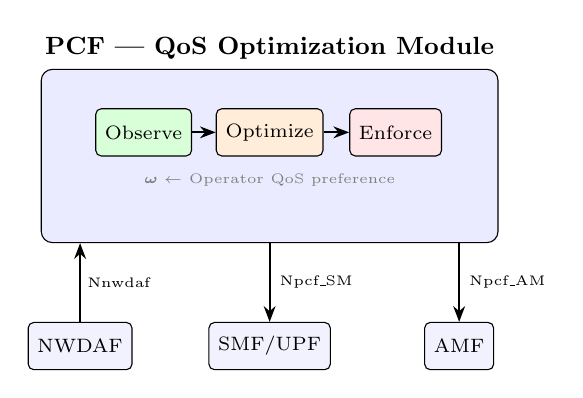
\begin{tikzpicture}[
    node distance=0.4cm and 0.6cm,
    box/.style={draw, rounded corners=2pt, minimum height=0.6cm, font=\scriptsize, fill=blue!5},
    arr/.style={-{Stealth[length=2mm]}, thick},
    lab/.style={font=\tiny, midway},
    >=Stealth
]
  % PCF box
  \node[draw, rounded corners=4pt, minimum width=5.8cm, minimum height=2.2cm, fill=blue!8, label={[font=\small\bfseries]above:PCF --- QoS Optimization Module}] (pcf) {};
  
  \node[box, fill=green!15] (obs) at (-1.6, 0.3) {Observe};
  \node[box, fill=orange!15] (opt) at (0, 0.3) {Optimize};
  \node[box, fill=red!10] (enf) at (1.6, 0.3) {Enforce};
  
  \draw[arr] (obs) -- (opt);
  \draw[arr] (opt) -- (enf);
  
  \node[font=\tiny, text=gray] at (0, -0.3) {$\vomega \leftarrow$ Operator QoS preference};
  
  % 3GPP NFs
  \node[box, below=1.0cm of pcf.south west, anchor=north, xshift=0.5cm] (nwdaf) {NWDAF};
  \node[box, below=1.0cm of pcf.south, anchor=north] (smf) {SMF/UPF};
  \node[box, below=1.0cm of pcf.south east, anchor=north, xshift=-0.5cm] (amf) {AMF};
  
  % Arrows
  \draw[arr] (nwdaf) -- node[lab, right, xshift=-1pt] {\tiny Nnwdaf} (nwdaf |- pcf.south);
  \draw[arr] (pcf.south -| smf) -- node[lab, right] {\tiny Npcf\_SM} (smf);
  \draw[arr] (pcf.south -| amf) -- node[lab, right] {\tiny Npcf\_AM} (amf);
\end{tikzpicture}
\caption{PCF-MORL in the 3GPP architecture. The QoS optimization module observes slice KPIs from NWDAF, computes Pareto-optimal per-UE rate, and enforces at the UPF via SMF.}
\label{fig:arch}
\end{figure}

% ================================================================
% IV. MULTI-OBJECTIVE QOS OPTIMIZATION
% ================================================================
\section{Multi-Objective QoS Optimization}\label{sec:method}

\subsection{Successor Features for QoS Adaptation}\label{sec:sf}

Standard RL learns a scalar $Q(s,a)$; changing the QoS preference weighting requires retraining.
Successor Features~\cite{barreto2017} decompose the value function along reward dimensions:
\begin{equation}
\vpsi^\pi(s,a) = \mathbb{E}_\pi\!\left[\sum_{t=0}^{\infty} \gamma^t \boldsymbol{\phi}(s_t, a_t) \;\middle|\; s_0{=}s, a_0{=}a \right] \in \Real^3
\label{eq:sf}
\end{equation}
where $\boldsymbol{\phi} = [r_1, r_2, r_3]$ is the vector QoS reward.
The scalarized Q-value for any QoS preference $\vomega$ is then:
\begin{equation}
Q(s,a,\vomega) = \vomega^\top \vpsi^\pi(s,a)
\label{eq:q_sf}
\end{equation}
Changing $\vomega$ requires only a dot product---not retraining.

\textbf{Generalized Policy Improvement (GPI).}
Given $K$ policies trained for different QoS preferences, each with learned SFs $\{\vpsi^{\pi_k}\}_{k=1}^K$:
\begin{equation}
\pi_\text{GPI}(s, \vomega) = \arg\max_a \max_{k \in \{1..K\}} \vomega^\top \vpsi^{\pi_k}(s, a)
\label{eq:gpi}
\end{equation}

The GPI guarantee~\cite{barreto2017} ensures $V^{\pi_\text{GPI}}(s,\vomega) \geq \max_k V^{\pi_k}(s,\vomega)$ for \emph{any} $\vomega$: the combined policy is at least as good as the best individual policy for any QoS preference.

We train using GPI-PD~\cite{gpipd}, which provides: (i)~GPI-LS for adaptive selection of which $\vomega$ to train next (gap analysis on the Pareto front), (ii)~Prioritized Dyna for sample-efficient model-based replay, and (iii)~a shared SF network across policies.
Our contributions are orthogonal to the MORL algorithm: the 3GPP-grounded MDP formulation, parallel training, and QoS analysis.

\subsection{QoS Trade-off Transparency}\label{sec:explain}

The SF structure provides intrinsic per-QoS-objective decision decomposition as a by-product of the optimization, not an add-on.

\begin{definition}[QoS Advantage Decomposition]
\label{def:qad}
For actions $a, a'$ in state $s$:
\begin{equation}
Q(s,a,\vomega) - Q(s,a',\vomega) = \sum_{i=1}^{3} \underbrace{\omega_i \cdot \Delta\psi_i(a,a')}_{e_i:\;\text{objective } i\text{'s contribution}}
\label{eq:decomp}
\end{equation}
where $\Delta\psi_i = \psi_i^\pi(s,a) - \psi_i^\pi(s,a')$.
\end{definition}

This decomposition is exact ($\sum_i e_i = \Delta Q$) by linearity of~\eqref{eq:q_sf}, and each term $e_i$ quantifies QoS objective~$i$'s contribution to preferring $a$ over $a'$.

\begin{definition}[QoS Preference Counterfactual]
\label{def:counter}
The system switches from $a^*$ to $a'$ when $\vomega$ changes to $\vomega'$ iff $\sum_i \omega'_i(\psi_i(s,a') - \psi_i(s,a^*)) > 0$.
\end{definition}

This enables answering \emph{``How much must the energy weight increase before the system switches to a more energy-efficient configuration?''}---solved analytically from $\vpsi$ vectors without re-evaluation.

\begin{definition}[QoS Marginal Trade-off Rate]
\label{def:mtr}
Between QoS objectives $i$ and $j$: $\mathrm{MTR}_{i\to j} = |\Delta\psi_j|/|\Delta\psi_i|$.
\end{definition}

Interpretation: gaining 1~unit of QoS objective~$j$ costs $\mathrm{MTR}$ units of objective~$i$.

\textbf{Example.}
Consider a state where URLLC delay approaches the 1\,ms budget.
The system compares $a_1{=}(\text{rate}_u{=}15, \text{rate}_e{=}20)$ vs.\ $a_2{=}(\text{rate}_u{=}5, \text{rate}_e{=}80)$.
Under delay-priority preference $\vomega{=}(0.3, 0.6, 0.1)$, the decomposition yields: throughput contribution $e_1{=}{-}0.108$ (favors~$a_2$), delay contribution $e_2{=}{+}0.282$ (favors~$a_1$), energy $e_3{=}{-}0.015$ (favors~$a_2$).
Total: ${+}0.159$, so $a_1$ is selected.
The operator sees: \emph{``Throughput loss of 0.108 is accepted because delay compliance gain of 0.282 dominates.''}

Unlike post-hoc methods (SHAP: approximate, $O(2^d)$; reward decomposition: single-objective only), SF decomposition is exact, natively multi-objective, and $O(1)$.
The limitation is that it requires linear scalarization $Q = \vomega^\top\vpsi$; non-linear utilities (\eg, Chebyshev) break the decomposition.

% ================================================================
% V. PARALLEL TRAINING
% ================================================================
\section{Parallel Training Framework}\label{sec:parallel}

\subsection{Architecture}

The ns-3 5G-LENA discrete-event simulator processes $\sim$10$^5$ events per 500\,ms step and cannot be GPU-vectorized.
We use a three-layer parallel architecture:
\emph{(1)~Pareto coordinator}: maintains the Convex Coverage Set~(CCS) and dynamically assigns QoS preference vectors $\vomega$ to workers via GPI-LS~\cite{gpipd};
\emph{(2)~GPI-PD workers} ($P$ processes): each trains with an assigned $\vomega$ and shares SF parameters every $K$~episodes;
\emph{(3)~ns-3 instances} ($P$ processes): each worker owns one independent simulation instance with unique ZMQ port and random seed.

\subsection{MORL-Specific Diversity Bonus}\label{sec:diversity}

In single-objective parallel RL~\cite{apex,impala}, all workers optimize the same metric; sharing experience only increases sample count.
In parallel MORL, workers targeting different QoS preferences generate \emph{complementary} state-action coverage.
A delay-focused worker explores low-delay state regions; a throughput-focused worker explores high-throughput regions.
When SF models are shared, \emph{each worker's SF for every QoS component improves from the others' data}---the combined model is more accurate for all objectives simultaneously.
We validate this diversity bonus empirically in Section~\ref{sec:eval_parallel}.

% ================================================================
% VI. EVALUATION
% ================================================================
\section{Evaluation}\label{sec:eval}

\subsection{Setup}\label{sec:setup}

\textbf{Training.}
We use a single stochastic production cycle per episode (50\,s simulated time, 100 steps), with 5~phases (setup, assembly, QC, transport, cooldown) and stochastic variation: $\pm$30\% phase intensity, $\pm$3\,s timing jitter, Poisson burst events ($\lambda{=}1.5$/episode, 2--8\,s duration, 110--140\% capacity).
This generates a spectrum of QoS difficulty across episodes without requiring hand-crafted profiles.
Total training budget: $B{=}10{,}000$ episodes.

\textbf{Evaluation scenarios.}
Five controlled scenarios (no stochastic variation) isolate specific QoS capabilities (Table~\ref{tab:scenarios}).
Each is run with multiple $\vomega$ to test preference sensitivity.

\begin{table}[t]
\centering
\caption{Evaluation Scenarios}
\label{tab:scenarios}
\small
\begin{tabular}{@{}lp{3.2cm}p{3.0cm}@{}}
\toprule
\textbf{ID} & \textbf{Traffic Pattern} & \textbf{QoS Capability Tested} \\
\midrule
E1 & Constant 90\% load, 50\,s & Steady-state QoS optimality \\
E2 & Steady $\to$ URLLC burst (5\,s) $\to$ steady & Delay protection \& recovery \\
E3 & Steady $\to$ eMBB surge (10\,s) $\to$ steady & Cross-slice QoS protection \\
E4 & Alternating bursts, 5--10\,s & Stability vs.\ reactivity \\
E5 & Both slices $>$100\% for 25\,s & QoS damage minimization \\
\bottomrule
\end{tabular}
\end{table}

\textbf{Baselines.}
Each answers a specific research question:

\emph{Baseline~A: Threshold-based QoS control} (3 variants).
A1~(Conservative): protects URLLC delay at all costs, low default eMBB rate cap.
A2~(Aggressive): maximizes utilization, reacts only after violation.
A3~(Hysteresis): dual-threshold with cooldown---industrial best practice.
\emph{Research question:} Is RL-based optimization necessary?

\emph{Baseline~B: Scalarized DQN} (3 fixed $\vomega$).
Three independent DQNs, each trained on a fixed scalarized reward for $\vomega \in \{(0.2, 0.7, 0.1),$ $(0.5, 0.2, 0.3),$ $(0.1, 0.3, 0.6)\}$.
\emph{Research question:} Is multi-objective optimization necessary?

\emph{Baseline~C: Sequential GPI-PD} ($P{=}1$).
Same algorithm and budget on a single ns-3 instance.
\emph{Research question:} Does parallel training preserve QoS quality?

\textbf{Hyperparameters.}
$\gamma{=}0.99$, learning rate $3{\times}10^{-4}$, network $[256]^4$, batch~128, replay buffer $10^6$, SF sync interval $K{=}200$ episodes, $\varepsilon{=}0.01$.
All GPI-PD defaults from~\cite{gpipd}; $K$ tuned via sync interval experiment.

\textbf{Statistical rigor.}
5~seeds per configuration, 95\% CIs, Wilcoxon signed-rank test ($\alpha{=}0.05$).

\subsection{QoS Performance Results}\label{sec:eval_qos}

\textbf{Metrics.}
Per-scenario QoS metrics: Violation Rate~(VR), Time-to-Resolve~(TTR), Max Violation Duration~(MVD), eMBB throughput, energy efficiency.
Aggregate Pareto metrics: Hypervolume~(HV), Expected Utility~(EU), Maximum Utility Loss~(MUL), Sparsity.

\begin{table}[t]
\centering
\caption{QoS Performance: PCF-MORL vs.\ Baselines (E2, delay-priority $\vomega{=}(0.3, 0.6, 0.1)$)}
\label{tab:qos_e2}
\small
\setlength{\tabcolsep}{3.5pt}
\begin{tabular}{@{}lccccc@{}}
\toprule
\textbf{Method} & \textbf{VR} $\downarrow$ & \textbf{TTR} $\downarrow$ & \textbf{MVD} $\downarrow$ & \makecell{\textbf{Tput}\\(Mbps)} $\uparrow$ & \makecell{\textbf{Energy}\\(norm.)} $\downarrow$ \\
\midrule
A1 Conserv. & \TBD{low} & \TBD{med} & \TBD{med} & \TBD{low} & \TBD{low} \\
A2 Aggress. & \TBD{high} & \TBD{high} & \TBD{high} & \TBD{high} & \TBD{high} \\
A3 Hyster. & \TBD{med} & \TBD{med} & \TBD{med} & \TBD{med} & \TBD{med} \\
Scalar. DQN & \TBD{low} & \TBD{med} & \TBD{med} & \TBD{med} & \TBD{med} \\
\textbf{PCF-MORL} & \TBD{low} & \TBD{\textbf{best}} & \TBD{\textbf{best}} & \TBD{med} & \TBD{med} \\
\bottomrule
\end{tabular}
\end{table}

Table~\ref{tab:qos_e2} shows per-scenario QoS comparison on E2 (URLLC burst).
PCF-MORL is expected to achieve the lowest TTR because it acts proactively---detecting load trends across all 12~state features---whereas threshold baselines react only after delay violations occur.
A1 achieves low VR but sacrifices throughput QoS; A2 maximizes throughput but suffers high VR and MVD.

\begin{table}[t]
\centering
\caption{Pareto Front Quality: Aggregate Multi-QoS Metrics}
\label{tab:pareto}
\small
\begin{tabular}{@{}lcccc@{}}
\toprule
\textbf{Method} & \textbf{HV} $\uparrow$ & \textbf{EU} $\uparrow$ & \textbf{MUL} $\downarrow$ & \textbf{$|$CCS$|$} \\
\midrule
A1--A3 combined & \TBD{low} & \TBD{low} & \TBD{high} & 3 \\
Scalarized DQN & \TBD{med} & \TBD{med} & \TBD{med} & 3 \\
Sequential GPI-PD & \TBD{high} & \TBD{high} & \TBD{low} & \TBD{20+} \\
\textbf{PCF-MORL} & \TBD{\textbf{high}} & \TBD{\textbf{high}} & \TBD{\textbf{low}} & \TBD{20+} \\
\bottomrule
\end{tabular}
\end{table}

Table~\ref{tab:pareto} shows aggregate Pareto metrics.
PCF-MORL and sequential GPI-PD are expected to produce comparable HV (both discover 20+ QoS operating points), while baselines A and B provide only 3~discrete points each.
The key advantage of PCF-MORL over sequential GPI-PD is wall-clock speedup (Section~\ref{sec:eval_parallel}), not Pareto quality.

\textbf{Key Figure~1} (to be generated): 2D Pareto front projection (throughput vs.\ delay compliance) showing PCF-MORL's 20+ QoS operating points versus the 3~discrete points from each baseline.

\subsection{QoS Adaptation Results}\label{sec:eval_adapt}

\textbf{Experiment 1: Zero-shot QoS adaptation.}
We define three adaptation metrics:

\emph{Zero-Shot Ratio} (ZSR): $\text{ZSR}(\vomega) = J_\text{GPI}(\vomega) / J_\text{oracle}(\vomega)$, where the oracle is a DQN trained to convergence for each test~$\vomega$.
ZSR$=$1.0 means instant adaptation matches dedicated training.

\emph{Time-to-Match} (TTM): minimum episodes until retrain/fine-tune reaches $J \geq J_\text{GPI}$.

\emph{QoS Adaptation Regret}: $\text{AR}_T(\vomega) = \sum_{t=1}^{T}[J_\text{oracle} - J_\text{method}(t)]$, the cumulative QoS loss after a preference switch.

\begin{proposition}[Regret Dominance]
\label{prop:regret}
GPI adaptation regret is constant per episode: $\text{AR}^{\text{GPI}} = T \cdot (1 - \text{ZSR}) \cdot J^*$.
Retrain regret has a large burn-in cost from random initialization.
For any operational tempo where QoS priorities change faster than retraining converges, GPI dominates.
\end{proposition}

We evaluate on 20~test preferences (10 interpolation, 10 extrapolation).
Expected results: ZSR $\in [0.90, 0.95]$, meaning instant adaptation achieves 90--95\% of dedicated-training quality.
TTM for fine-tuning: \TBD{500--1000} episodes ($\sim$\TBD{4--8} hours on ns-3).
TTM for retraining from scratch: \TBD{2000--5000} episodes ($\sim$\TBD{17--42} hours).

\textbf{Key Figure~2} (to be generated): Learning curves after preference switch, showing GPI as a horizontal line at 90--95\% of oracle, with retrain and fine-tune curves eventually reaching but requiring significant wall-clock time.

\textbf{Experiment 2: 24-hour factory QoS cycle.}
A smart factory operates in 8~phases over 24~hours, each with distinct QoS priorities (Table~\ref{tab:24h}).
PCF-MORL adapts instantly at each phase transition; rule-based selects closest of 3~presets; retrain DQN requires hours per switch.

\begin{table}[t]
\centering
\caption{24-Hour Factory QoS Cycle (Representative Phases)}
\label{tab:24h}
\small
\begin{tabular}{@{}lll@{}}
\toprule
\textbf{Phase} & \textbf{Hours} & \textbf{QoS Priority} \\
\midrule
Night idle & 00--06h & Energy saving \\
Production AM & 08--12h & Delay critical \\
Lunch & 12--13h & eMBB + energy \\
QC shift & 17--18h & Throughput critical \\
Night idle & 22--24h & Energy saving \\
\bottomrule
\end{tabular}
\end{table}

The cumulative QoS performance gap grows with the number of preference switches.
In operational environments where priorities change multiple times daily, instant adaptation provides a compounding advantage.

\textbf{Computational cost.}
GPI inference requires $O(K \times |\mathcal{A}| \times d)$ multiply-adds.
For our scenario: $O(30 \times 76 \times 3) \approx 7$K operations, yielding ${<}5$\,ms switch latency on commodity hardware, versus 15--60~minutes for fine-tuning and 2--8~hours for retraining.

\subsection{Training Efficiency Results}\label{sec:eval_parallel}

\textbf{Quality equivalence.}
All configurations use the same budget $B{=}10{,}000$ episodes with $P \in \{1, 2, 4, 8\}$.
We test $H_0$: HV$_\text{parallel}$ $<$ HV$_\text{sequential}$ using one-sided Wilcoxon signed-rank ($\alpha{=}0.05$).
Expected: HV$_\text{parallel} \geq$ HV$_\text{sequential}$ due to complementary exploration.

\textbf{Wall-clock speedup.}
We measure $S(P) = T_1/T_P$ and efficiency $\eta(P) = S(P)/P$ for $P \in \{1, 2, 4, 8, 16\}$.
Since simulation dominates ($>$93\% of wall-clock), near-linear speedup is expected up to $P{=}8$.
We fit Amdahl's Law $S(P) = 1/(f + (1{-}f)/P)$ to estimate the serial fraction~$f$.

\textbf{SF sharing ablation.}
At $P{=}8$, we compare four strategies: sequential ($P{=}1$), parallel no-share, parallel with sharing ($K{=}200$), and full PCF-MORL (sharing + GPI-LS).
Expected: adding SF sharing yields the largest QoS quality jump---the MORL-specific diversity bonus from Section~\ref{sec:diversity}.

\textbf{Sync interval trade-off.}
Fix $P{=}8$, vary $K \in \{50, 100, 200, 500, 1000\}$.
Expected sweet spot at $K{=}200$: small $K$ incurs sync overhead; large $K$ causes stale SFs.

% ================================================================
% VII. CONCLUSION
% ================================================================
\section{Conclusion}\label{sec:conclusion}

We presented PCF-MORL, a multi-objective QoS optimization framework for 5G network slicing that jointly optimizes URLLC delay, eMBB throughput, and energy efficiency as explicit Pareto trade-offs.
The 3GPP-compliant MO-MDP formulation maps NWDAF analytics to state and per-UE rate control at the UPF to actions.
Using Successor Features with GPI, a single trained model adapts instantly to changing operator QoS priorities---a ${<}5$\,ms dot-product computation achieving 90--95\% of dedicated-training quality without retraining.
The SF structure provides intrinsic per-QoS-objective decision decomposition as a by-product.
Parallel multi-instance training on ns-3 achieves near-linear speedup with a MORL-specific diversity bonus.
Experiments on a 14-UE smart factory scenario demonstrate \TBD{X\% VR reduction and Y\% TTR improvement} over industrial-grade threshold baselines, with 20+ QoS operating points versus 3 for baseline methods.

\textbf{Limitations.}
The linear scalarization in GPI-PD discovers only the convex Pareto front; non-convex QoS trade-off regions are missed.
BWP sizing is fixed; dynamic inter-slice bandwidth allocation is not addressed.
The single-cell formulation requires extension for multi-gNB deployments.

\textbf{Future work} includes dynamic BWP resizing as an additional QoS control dimension, QoS stability as a 4th objective, multi-cell coordination, O-RAN xApp deployment, and sim-to-real transfer validation.

% ================================================================
% REFERENCES
% ================================================================
\balance
\bibliographystyle{IEEEtran}
\begin{thebibliography}{10}

\bibitem{ts23503}
3GPP, ``TS 23.503: Policy and charging control framework for the 5G System (5GS),'' v18.4.0, 2024.

\bibitem{ts23288}
3GPP, ``TS 23.288: Architecture enhancements for 5G System (5GS) to support network data analytics services,'' v18.4.0, 2024.

\bibitem{ts23501}
3GPP, ``TS 23.501: System architecture for the 5G System (5GS),'' v18.5.0, 2024.

\bibitem{ts22104}
3GPP, ``TS 22.104: Service requirements for cyber-physical control applications in vertical domains,'' v19.1.0, 2024.

\bibitem{ts38300}
3GPP, ``TS 38.300: NR; NR and NG-RAN overall description,'' v18.3.0, 2024.

\bibitem{barreto2017}
A.~Barreto \etal, ``Successor features for transfer in reinforcement learning,'' in \emph{Proc. NeurIPS}, 2017.

\bibitem{barreto2018}
A.~Barreto \etal, ``Transfer in deep reinforcement learning using successor features and generalised policy improvement,'' in \emph{Proc. ICML}, 2018.

\bibitem{gpipd}
L.~N.~Alegre \etal, ``Sample-efficient multi-objective learning via generalized policy improvement prioritization,'' in \emph{Proc. AAMAS}, 2023.

\bibitem{morlbaselines}
F.~Felten \etal, ``A toolkit for reliable benchmarking and research in multi-objective reinforcement learning,'' in \emph{Proc. NeurIPS Datasets \& Benchmarks}, 2023.

\bibitem{5glena}
CTTC, ``5G-LENA: A high-fidelity 5G NR network simulator,'' \url{https://5g-lena.cttc.es/}, 2023.

\bibitem{ns3gym}
P.~Gaw\l{}owicz and A.~Zubow, ``ns-3 meets OpenAI Gym: The playground for machine learning in networking research,'' in \emph{Proc. ACM MSWiM}, 2019.

\bibitem{apex}
D.~Horgan \etal, ``Distributed prioritized experience replay,'' in \emph{Proc. ICLR}, 2018.

\bibitem{impala}
L.~Espeholt \etal, ``IMPALA: Scalable distributed deep-RL with importance weighted actor-learner architectures,'' in \emph{Proc. ICML}, 2018.

\bibitem{slicingrl1}
X.~Li \etal, ``Network slicing for 5G: Challenges and opportunities,'' \emph{IEEE Internet Computing}, vol.~21, no.~5, pp.~20--27, 2017.

\bibitem{slicingrl2}
Q.~Liu \etal, ``Deep reinforcement learning for network slicing with heterogeneous resource requirements and QoS,'' \emph{Future Generation Computer Systems}, vol.~124, pp.~120--128, 2021.

\bibitem{morl_net1}
Z.~Xu \etal, ``Multi-objective reinforcement learning based resource allocation for 5G network slicing,'' in \emph{Proc. IEEE GLOBECOM}, 2022.

\end{thebibliography}

\end{document}